\documentclass[conference]{IEEEtran}
\usepackage{cite}
\usepackage{amsmath,amssymb,amsfonts}
\usepackage{algorithmic}
\usepackage{graphicx}
\usepackage{textcomp}
\usepackage{xcolor}
\def\BibTeX{{\rm B\kern-.05em{\sc i\kern-.025em b}\kern-.08em
    T\kern-.1667em\lower.7ex\hbox{E}\kern-.125emX}}
\begin{document}
\makeatletter
\newcommand{\linebreakand}{%
  \end{@IEEEauthorhalign}
  \hfill\mbox{}\par
  \mbox{}\hfill\begin{@IEEEauthorhalign}
}
\makeatother

\title{Comparative Study of Voice-Activated vs Controller-Based Manipulation in Pick-and-Place Robotics\\
}

\author{\IEEEauthorblockN{Neel Girish Bahadarpurkar}
\IEEEauthorblockA{\textit{MS Robotics Engineering} \\
\textit{Worcester Polytechnic Institute}\\
Worcester, Massachusetts\\
nbahadarpurkar@wpi.edu}
\and
\IEEEauthorblockN{Harshal Suresh Bhat}
\IEEEauthorblockA{\textit{MS Robotics Engineering} \\
\textit{Worcester Polytechnic Institute}\\
Worcester, Massachusetts \\
hbhat@wpi.edu}
\and
\IEEEauthorblockN{Brendan Byrne}
\IEEEauthorblockA{\textit{BS Robotics Engineering \& Computer Science} \\
\textit{Worcester Polytechnic Institute}\\
Marshfield, Massachusetts \\
bsbyrne@wpi.edu}
\linebreakand
\IEEEauthorblockN{Jack Lynch}
\IEEEauthorblockA{\textit{MS Computer Science} \\
\textit{Worcester Polytechnic Institute}\\
Shrewsbury, Massachusetts \\
jmlynch@wpi.edu}
\and
\IEEEauthorblockN{Paul Raynes}
\IEEEauthorblockA{\textit{MS Robotics Engineering} \\
\textit{Worcester Polytechnic Institute}\\
Worcester, Massachusettes \\
psraynes@wpi.edu}
}

\maketitle

\begin{abstract}
This study compares the performance of voice instructions against mechanical controls in a simulated work setting. Participants in a Unity-based simulation are charged with commanding autonomous robots to fetch certain things using mechanical controllers or vocal instructions. The NASA-TLX approach is used in the experiment to assess job completion time and obtain user input on workload and preferences. The study intends to determine if voice control may improve productivity and usability in real-world applications, hence leading to a better understanding of human-robot interaction in industrial settings. 
\end{abstract}

\section{Introduction}
With autonomous robots becoming more prevalent in workplace settings, determining the most efficient means of commanding them becomes an important task. As human workers may have their own tasks to perform in addition to commanding the machines, finding an efficient control method that can reduce the overall workload of the human operator becomes important. Currently, mechanical controls are the most widespread, as they are both easy and cheap to implement. Another control method that has become more popular has been voice communication. While voice communication seems to be more efficient on paper, there can of course be issues in certain scenarios. Our project aims to determine if voice commands are preferable to normal basic commands in a work environment by creating a simulation with both mechanical and voice commands to determine which one people prefer.  

\section{Related Work}
Past research work has investigated the efficacy of various robot control techniques, focusing on the comparison between manual control and voice commands. Bremner and Leonards \cite{7139460}\cite{10.3389/fpsyg.2016.00183} examined the integration of speech and gestures for robotic communication. In contrast to manual control techniques, which need more direct and accurate input, their study revealed that mixing voice commands with gestures improves both robot likeability and efficiency, making interactions more intuitive for users. 

Comparing autonomous control to voice control, Vatsal and Hoffman \cite{8461212} investigated a wearable robotic forearm intended for cooperative tasks. Their research showed that although voice instructions had their uses, people preferred autonomous control when doing repeated and difficult activities since it was faster and more efficient. This implies that although voice instructions have their advantages, there are situations in which they might not be as effective as alternative approaches. 

A framework for classifying voice-controlled and manual human-robot conversation systems was created by Berzuk and Young in 2022\cite{9889423}. Their study demonstrated the benefits of multimodal communication (speech, gestures, etc.), demonstrating that in some situations, these systems perform better than only voice- or manual-based control because they allow for more flexible and adaptive interactions. 

Finally, in 2017, research from the CARIS lab \cite{evangelista2017grounding} showed that voice-controlled robots are now more widely available in industrial settings thanks to natural language commands, which greatly increase the usability of voice-controlled robots for non-expert users. This method contrasts with manual control methods, which demand more concentration and training.  

These studies highlight that although voice command systems provide a more natural interface, depending on the job complexity and user expectations, there are situations in which manual control or autonomous systems may provide greater performance or preference. This context guides our study's exploration of whether voice commands can function more effectively in a workplace setting than conventional mechanical controls. 

\section{Proposed Method}
To determine the effectiveness of voice controls in a supervisory control scheme, our method will compare voice controls to a typical mechanical control scheme. We will create a 3D task environment which will simulate a potential real-life usage for supervisory control in the Unity engine. This simulation will contain four rooms, one which the participant’s character in the simulation will work from, as well as three rooms which house three different autonomous agents, which all have an opening leading to the user’s room. The user will be unable to enter the robots’ rooms. Within each room will be nine objects, each with a unique shape and color combination that can be collected by the robots and brought to the user through the opening. Each of these shapes will be labelled 1 through 3 depending on which agent’s room it came from. There will also be nine unlabeled objects within the user’s room. Outside of each room will be a display which the user can use to control the robots mechanically.

\begin{figure}[htbp]
\centerline{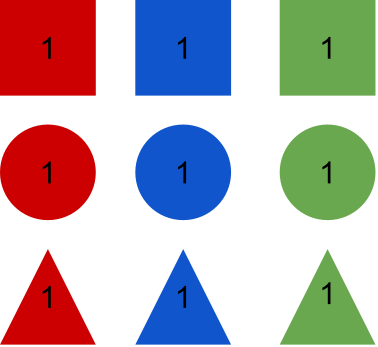
\includegraphics[width=0.45\textwidth]{sample_shapes_grid.png}}
\caption{Example of what the shapes will look like}
\label{sample_grid}
\end{figure}


\section{Experiment}
During the experiment, participants will be shown a sequence of shapes that they need to construct using an object from their room as well as one from the three adjacent rooms. As the participant cannot enter the adjacent rooms, they must command the agents to provide the correct objects for them. Once a set number of sequences are completed by the user, the time it took to accomplish the task will be recorded for evaluation.  

\begin{figure}[htbp]
\centerline{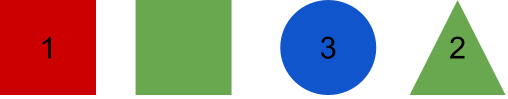
\includegraphics[width=0.45\textwidth]{sample_sequence.png}}
\caption{Example of a shape sequence}
\label{sample_sequence}
\end{figure}

There will be two versions of the simulation. The first version will use the displays found outside the rooms of the robots which the user will utilize to obtain the needed objects for the sequence. This will simulate typical mechanical controls for the automata. In the second version of the simulation, instead of the displays, voice commands will be used. Participants will be requested to speak into their microphones to request objects from one of the three robots. An example command could be “Robot 1, bring me the red square”.  

Evaluation of both methods will be conducted by comparing the times needed to complete the sequences in both the mechanical and voice activated trials. In addition to the time, feedback from the participants in the study will also be collected to analyze both workload levels as well as the overall user experience. A subjective usability test such as the NASA-TLX or a Likert scale will be used to collect this feedback. 

\section{Preliminary Results}
Our first deliverable 	for this project is a basic unity simulation which will be built upon to create our final simulation. Currently, the simulation is incredibly simple and only serves to be a foundation from which the rest of the simulation can be built upon. This simulation features a rectangular block which acts as the robot and two platforms, a red one on the right and a blue one on the left. With the A and D keys, the block moves between the two platforms. This is to give an idea of how the robot will move between various objects and points. As the experiment will involve robots going between various points to pick up and deliver objects. 

As of right now, the movement is a bit buggy, as the block attempts to clip into the platform. This is a result of the MoveTowards function, which moves an object to the position of another object. However, this attempts to move the block to the center of mass of the platform, which causes a ‘clipping’ effect as the block attempts to move inside the platform. While this is merely a stylistic thing, it does have the potential to become an issue down the line if the robots are unable to make it to their destination due to this clipping. The chances of this becoming an issue is slim, but it is still worth mentioning as a possible issue.

The Hugging Face API for speech recognition was used to construct the block's voice control system, which allows for 2D movement with four basic commands: up, down, left, and right. These commands are converted into movements that move the block in two dimensions, providing easy, hands-free control. This approach streamlines interaction by removing the requirement for physical controllers, making it more user-friendly and efficient in certain job contexts. 
\section{Task Division \& Timeline}
\subsection{Schedule}
\begin{table}[htbp]
\begin{center}
\begin{tabular}{|c|c|c|}
\hline
\textbf{Task} & \textbf{Start Date} & \textbf{Due Date} \\
\hline
Make Unity Simulation Tests & Oct. 21st & Nov. 8th \\
\hline
Testing Phase & Nov. 8th & Nov. 15th \\
\hline
Data Analysis & Nov. 15th & Nov. 21th \\
\hline
1st Draft Presentation Slides & --- & Nov. 28th \\
\hline
Final Paper Review & --- & Dec. 1st \\
\hline
Final Paper Submitted \& Presented & --- & Nov. 2nd \\
\hline
\end{tabular}
\label{tab1}
\end{center}
\end{table}

\subsection{Task Division}
\begin{itemize}
\item Unity Development and Simulation: Developing the simulation environment for user interaction – Jack Lynch 
\item Voice Processing: Implement voice control systems for robotic manipulation – Neel Girish Bahadarpurkar, Harshal Suresh Bhat 
\item User Interface with Visual Cues: Designing visual feedback and user interaction cues – Paul Raynes 
\item Experiment Design \& Analysis: Organizing experimental tasks and analyzing data – Brendan Byrne 
\end{itemize}

\bibliographystyle{ieeetran}
\bibliography{project_proposal}

\end{document}
